\section{Ocean Dissipation in Titan \label{sec:results_Titan}}

The following results are split into three main sections. We firstly present specific solutions to the LTEs for a global surface ocean on Titan using Rayleigh friction. We then compare dissipation between the analytical and numerical solutions in section \ref{subsubsec:linTitan}. Section \ref{subsec:botTitan} then presents purely numerical results for dissipation using only bottom friction. These results are then repeated for Enceladus in section \ref{sec:results_Enceladus}.

\subsection{Rayleigh Friction}

\subsubsection{LTE Solutions}

Figure \ref{fig:LTE_solns} illustrates numerical solutions to the LTE, at periapse, for different components of the tidal potential on Titan. Surface displacement, $\eta$, is illustrated on the left, whereas velocity, $\bm{u}$, is on the right. The colour scale in the velocity figures represents the velocity's magnitude, $\left| \bm{u} \right|$. Arrows indicate the direction of flow. The tidal forcing applied is, from a) to c), the eccentricity tide, obliquity tide, and full tide, respectively. All plots are for the ``canonical'' $400 \, \si{\metre}$ ocean used by \citet{sagan1982tide} for best comparison with \citet{sears1994tidal,sears1995tidal,sohl1995tidal}.

Surface displacement in Figure \ref{fig:LTE_a} shows a classic tidal bulge, centered on the Saturnian ($\phi = 0^{\circ}$) and sub-Saturian ($\phi = 180^{\circ}$) points. Maximum displacement is over $8$ metres. Away from the tidal bulge, displacement drops below the equilibrium level to less than $4$ metres. The corresponding flow shows convergence and divergence at the longitudinal positions of steepest gradient in the displacement field. Fastest flow occurs at the maxima and minima of the displacement.

\begin{figure*}[!t]
    \centering
    \begin{subfigure}[t]{0.9\linewidth} % contains the two plots in a single figure
        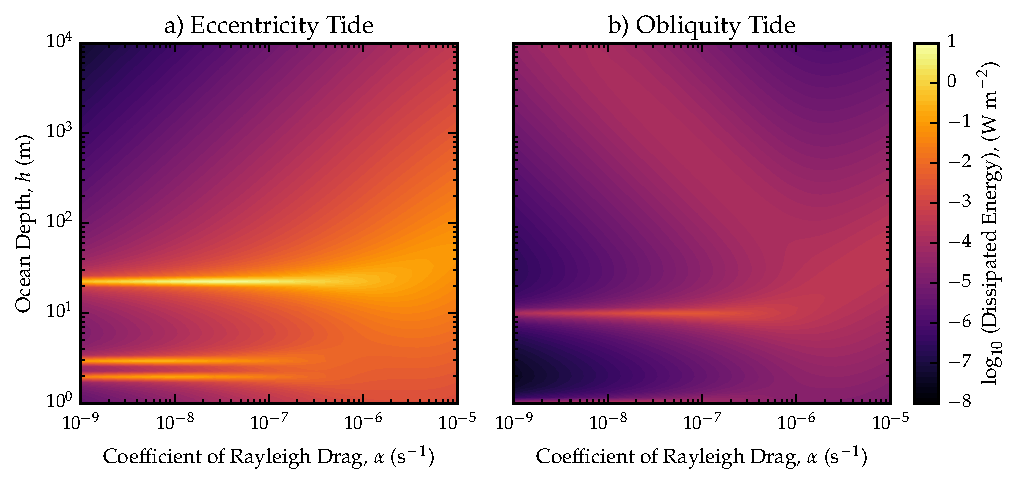
\includegraphics[width=\linewidth]{Figures/titan_linear}
        \phantomcaption
        \label{fig:lincEccTitan}
    \end{subfigure}
    \begin{subfigure}[t]{0\linewidth} % the hidden unwanted image
         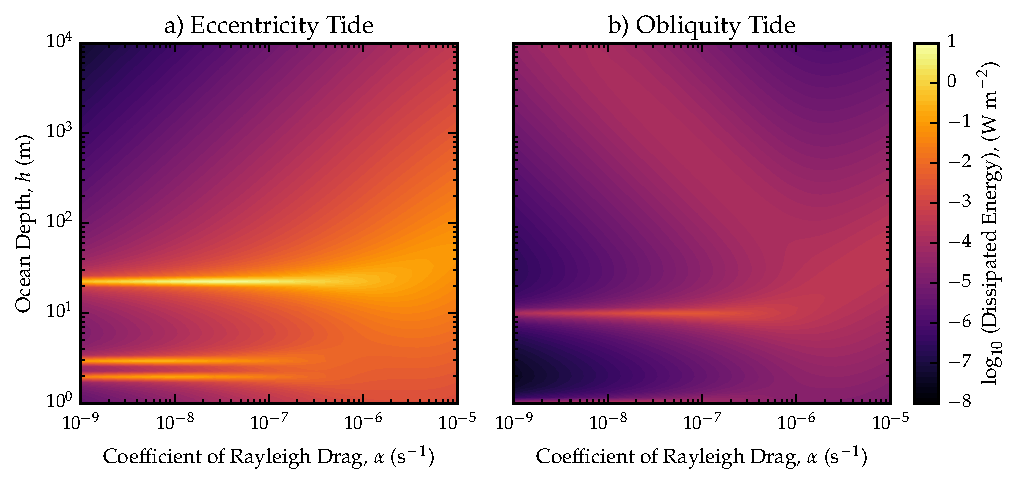
\includegraphics[width=\linewidth]{Figures/titan_linear}
         \phantomcaption
         \label{fig:linObliqTitan}   
    \end{subfigure}
    \vspace{-0.5cm}
\caption{Global ocean surface dissipation solution for Titan under the eccentricity (left) and obliquity (right) tides. The logarithm of dissipated energy is shown as a function of ocean depth, $h$, and Rayleigh friction coefficient, $\alpha$. All simulations were performed with \SIrange{2}{3}{\degree} resolution.}
\label{fig:linTitan}
\end{figure*}

The obliquity tide shows markedly different displacement and flow patterns than the eccentricity tide (Figure \ref{fig:LTE_b}). Displacement is now anti-symmetric about the equator. Notably, the longitudinal positions of maxima and minima are offset from the Saturnian and sub-Saturnian points. The tide raised by the obliquity tidal potential is also an order of magnitude less than the eccentricity tide. Flow is mainly poleward, converging south of the equator on the Saturn-facing hemisphere, and north of the equator on the opposite hemisphere.

The final plot in figure \ref{fig:LTE_solns} is the solution under the full tidal potential. In many ways it is similar to the eccentricity tide. Yet, the addition of the obliquity tide adds a degree of equatorial asymmetry to the solutions. This asymmetry is particularly noticeable in the velocity plot on the right hand side of Figure \ref{fig:LTE_c}, where the areas of fastest flow are skewed north and south of the equator, unlike in Figure \ref{fig:LTE_a}. This is also evident in the displacement field, where the highest tide is offset from the equator.

These simulations were run from undisturbed initial conditions: \hbox{$\eta = 0 \, \si{\metre}$} and \hbox{$\bm{u} = (0,0) \, \si{\metre\per\second}$}. Consequently, there was some start-up time required for the model to converge into its orbitally-averaged equilibrium, as noted by \citet{sears1995tidal}. Figure \ref{fig:conv_a} illustrates this type of behaviour.



\subsubsection{Tidal Dissipation \label{subsubsec:linTitan}}

Dissipated surface heat flux averaged over the tidal period was calculated for over 3000 simulations using equations \ref{eq:E_alpha} and \ref{eq:E_alpha_orbit}. These simulations were performed for a range of $h$ and $\alpha$ values for each main tidal component, as shown in Figure \ref{fig:linTitan}. The eccentricity tide (Figure \ref{fig:lincEccTitan}) shows three resonant dissipative ocean thicknesses, $h \sim$ \SIlist{2;3;22}{\metre}. These horizontal resonances are the result of excited gravity waves, with the deepest of these having a maximum dissipated surface heat flux of $\sim 10\, \si{\watt\per\square\metre}$ which occurs between $\alpha =$ \SIrange{e-8}{e-7}{\per\second}. Notably, the maximum dissipated energy does not occur for the most friction dominated oceans where $\alpha \sim \num{e-5} \, \si{\per\second}$. 


\begin{figure*}[!t]
    \centering
    \begin{subfigure}[t]{0.9\linewidth} % contains the two plots in a single figure
        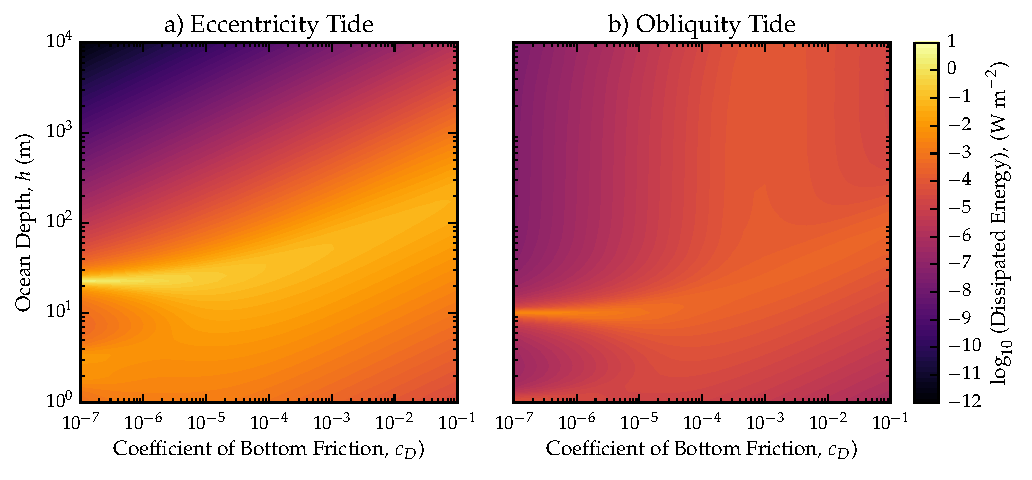
\includegraphics[width=\linewidth]{Figures/titan_bottom}
        \phantomcaption
        \label{fig:botEccTitan}
    \end{subfigure}
    \begin{subfigure}[t]{0\linewidth} % the hidden unwanted image
         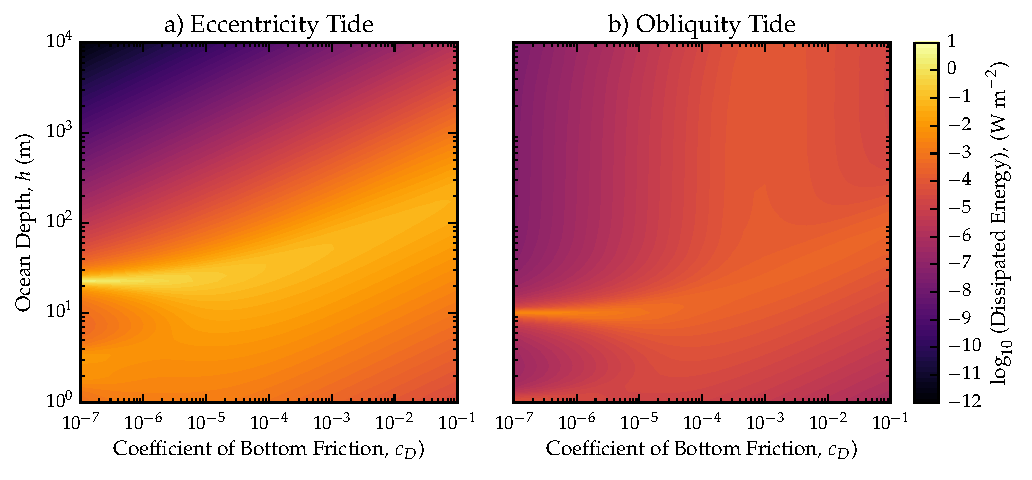
\includegraphics[width=\linewidth]{Figures/titan_bottom}
         \phantomcaption
         \label{fig:botObliqTitan}   
    \end{subfigure}
    \vspace{-0.5cm}
\caption{Global ocean surface dissipation solution for Titan under the eccentricity (left) and obliquity (right) tides. The logarithm of dissipated energy is shown as function of ocean depth, $h$, and coefficient of bottom friction, $c_D$. All simulations were performed with \SIrange{1}{3}{\degree} resolution. \label{fig:botTitan}}
\end{figure*}

Figure \ref{fig:lincEccTitan} illustrates the dissipated surface heat flux for the obliquity tide on Titan. Two resonant ocean thicknesses are found for this tidal component, $h \sim$ \SIlist{1;10}{\metre}. The latter resonance is the most dissipative with an average surface heat flux of $\sim \num{4e-3}\, \si{\watt\per\square\metre}$. There is also a slanted resonance that appears from $h \sim$ \SIrange{10}{e4}{\metre} and \hbox{$\alpha \sim$ \SIrange{e-6}{e-9}{\per\second}}. The average surface heat flux occurring along the length of this resonance is $\sim \num{1e-4}\, \si{\watt\per\square\metre}$. 

Numerical error was also computed using the analytical solutions. The eccentricity tide is accurate to within 1\% over much of the parameter space, with resonances being the least accurate (in terms of absolute value). The deepest resonance differs from the analytical solution by \SIrange{1}{20}{\percent}. We ignore discrepancies in shallow oceans ($h_0 \leq 10 \, \si{\metre}$); bathymetry of the ocean floor for any icy satellite will likely be comparable to or exceed the depth of the ocean, directly violating the assumptions made in the LTEs. It should also be noted that resonances found below $h_0 = 10 \, \si{\metre}$ typical have $\text{min} (\eta) < - h_0$, also violating the LTEs. As such, we deem this part of the parameter space unphysical.

\subsection{Bottom Friction \label{subsec:botTitan}}

Dissipation across $h$ and $c_D$ space (bottom friction) is shown in Figure \ref{fig:botTitan}, again calculated using equations \ref{eq:E_cd} and \ref{eq:E_cd_orbit}. Tidal dissipation due to the eccentricity tide is shown in the left hand figure. Comparing this to Rayleigh dissipation in Figure \ref{fig:lincEccTitan} highlights some of the major differences and similarities between the two friction regimes. The resonant peaks at \SIlist{2;3;22}{\metre} from the Rayleigh friction case are all present, although they have smaller magnitudes. The resonance broadens towards larger $c_D$, and remains very diffuse over much of the parameter space. This differs from the Rayleigh friction case where the resonances is very narrow and pronounced over most of $\alpha$ space (Figure \ref{fig:lincEccTitan}). Additionally, away from the resonances and in the deepest oceans, dissipated energy drops by \numrange{10}{12} orders of magnitude when applying bottom friction, which is far smaller than the lowest dissipation found in the Rayleigh friction case.  

Ocean dissipation under the obliquity tide using bottom friction also has several important differences to the Rayleigh friction case. Comparing figures \ref{fig:botObliqTitan} and \ref{fig:linObliqTitan}, it is again evident that the horizontal gravity wave resonances at \SIlist{1;10}{\metre} are still present when using bottom friction. These resonances rapidly broaden towards higher $c_D$, when bottom drag becomes more dominant. Perhaps the most significant difference between each case is the orientation of the broad resonance that extends to the deepest oceans. In the Rayleigh case, this resonance moves diagonally across a large region of the parameter space, whereas it is vertically oriented and limited to a small range of $c_D$ for bottom friction. The resonance also happens to occur across the empirically derived Earth value for $c_D = 0.002$ \citep[e.g.,][]{sohl1995tidal,egbert2001estimates}.

\subsection{Comparison with Scaling Laws \label{subsec:scalTitan}}

While there are no fully analytical solutions to the LTEs when including bottom friction, there are a set of scaling laws for estimating dissipation that neglect resonant features, developed by \citet{chen2013tidal}. We compare cross sections from the results in Figure \ref{fig:botTitan} with these scaling laws, shown in Figure \ref{fig:scalTitan}.

\begin{figure*}[!t]
\centering
\begin{subfigure}{0.4\linewidth}
\centering
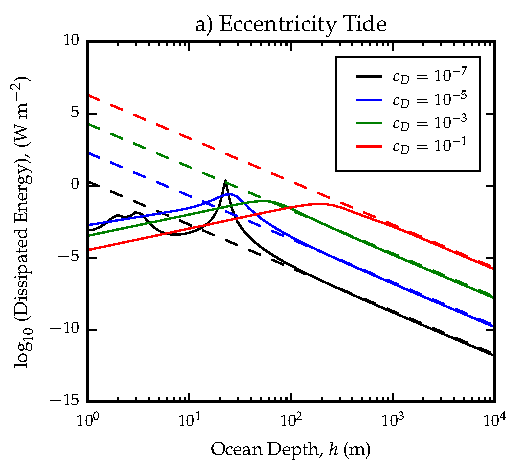
\includegraphics[width=\linewidth]{Figures/Eccentricity_scaling}
\subcaption{\label{fig:scalEccTitan}}
\end{subfigure}%
\begin{subfigure}{0.4\linewidth}
\centering
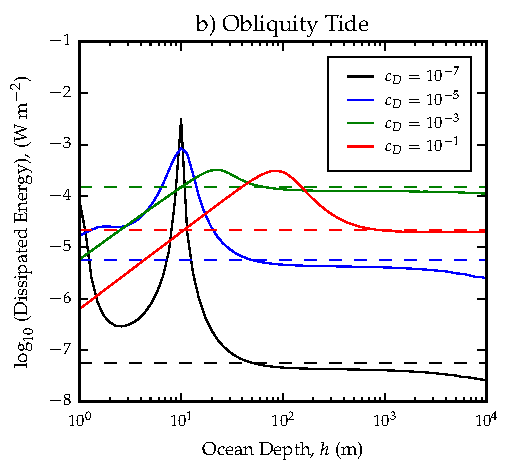
\includegraphics[width=\linewidth]{Figures/Obliquity_scaling}
\subcaption{\label{fig:scalObliqTitan}}
\end{subfigure}
\vspace*{-0.8cm}
\caption{Comparison of the ODIS numerical results (solid lines) and those calculated using the scaling laws (dashed lines) derived in \citet{chen2013tidal}, for Titan. There is excellent agreement between the two results for deep oceans and away from resonances. \label{fig:scalTitan}}
\end{figure*}

Away from resonances and in deep oceans, there is excellent agreement between the numerical ODIS results and the scaling laws. This is particularly true of the eccentricity tide. Larger discrepancies are found for the obliquity tide (Figure \ref{fig:scalObliqTitan}) for large ocean depths, but this is a result of discretisation error. The vertically orientated resonant feature in Figure \ref{fig:botObliqTitan} is also recreated in the scaling laws shown in Figure \ref{fig:scalObliqTitan}. None of the gravity wave resonances are captured by the scaling laws. 

\subsection{Implications for Titan}

\begin{figure*}[!t]
\centering
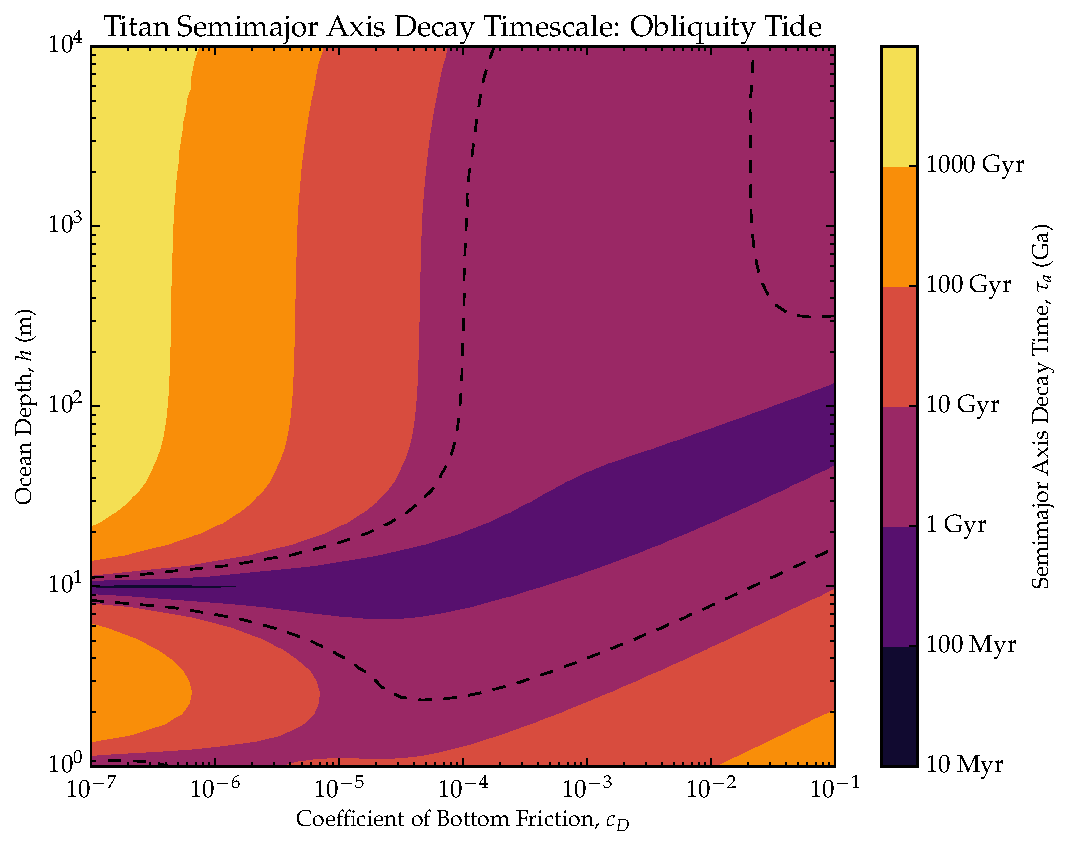
\includegraphics[width=0.5\linewidth]{Figures/a_decay}
\caption{Comparison of the ODIS numerical results (solid lines) and those calculated using the scaling laws (dashed lines) derived in \citet{chen2013tidal}, for Titan. There is excellent agreement between the two results for deep oceans and away from resonances. \label{fig:a_evo}}
\end{figure*}

Titan likely has an ocean that is several hundred kilometres thick \citep{sohl2003interior}. All of the eccentricity tide resonances occur at ocean depths much more shallow than this, suggesting that - despite the substantial free eccentricity - there is little dissipation from this tidal component in heating Titan's ocean.

Rossby wave resonances from the obliquity tide appear as the diagonal and vertical features in figures \ref{fig:linObliqTitan} and \ref{fig:botObliqTitan}, respectively. The linear friction resonance moves into unrealistically low coefficients of friction ($\alpha \lesssim$ \SI{e-9}{\per\second}) for oceans deeper than about \SI{10}{\kilo\metre}. However, for bottom friction, the Rossby wave resonance is mainly independent of ocean depth above $h \gtrsim$ \SI{100}{\metre}. If Titan's ocean fell within the $c_D =$ \SIrange{e-2}{e-4} range then this Rossby wave resonance could provide a non-neglible thermal energy component to Titan's interior, regardless of the ocean depth. To gain some insight into how significant this dissipation can be, we consider some upper limits of Titan's semimajor axis evolution.

Hyperion is the next furthest satellite from Saturn after Titan, with a semimajor axis  $1.21 a$ \citep{sears1995tidal}. Titan would have to have originated at some semimajor axis less than Hyperion's, otherwise Hyperion would have been disturbed or ejected from the system, assuming Hyperion and Titan have similar ages. This provides us with a useful upper bound for Titan's  initial semimajor axis. Using the dissipated energy results for the obliquity tide under bottom friction, we can examine how rapidly Titan's semimajor axis shrinks to its present day value.

For a bound orbit the total energy is given as $-GMm/2a$ \citep{goldreich1966q}. Differentiating this expression with respect to time gives a relationship between the dissipated energy and changing semimajor axis,
\begin{equation}
\dot{a} = \dfrac{2a^2 \dot{E}}{GM m}.
\label{eq:adot}
\end{equation}

where $M$ and $m$ represent the mass of Saturn and Titan, respectively. The universal gravitational constant is $G$, and dissipated energy in watts is $\dot{E}$. Note that as $\dot{E} < 0$, the semimajor axis decays with time. To first order, $\dot{E}$ remains mostly constant over the range $1.21 a$ to $a$ for a deep ocean on Titan undergoing bottom friction for the obliquity tide. This is because the position of the vertical Rossby wave resonance (Figure \ref{fig:botObliqTitan}) is only weakly sensitive to the rotation rate of Titan, which varies from $\Omega =$ \SIrange{4.56e-6}{3.42e-6}{\per\second} over the range of semimajor axes that we consider, assuming synchronous rotation. Additionally, it should be noted that while $\dot{E}$ is rather more sensitive to the acutal obliquity, $\theta_0$, we set this to constant for simplicity. A more rigorous (and future) approach would include this coupling.

We integrate Equation \ref{eq:adot} to estimate the evolution of Titan's semimajor axis as a function of time and dissipated energy, defining a characteristic semimajor axis decay time, $\tau_{a}$, as the time taken for the semimajor axis to reach its present day value from Hyperion's semimajor axis. The decay time as a function of ocean depth and bottom friction coefficient is shown in Figure \ref{fig:a_evo}.
  
As expected, the smallest $\tau_a$ occurs for the largest dissipation, namely the gravity wave resonance at \SI{10}{\metre}, with decay times on the order of \SI{100}{\mega\year}. However, as previously mentioned, Titan's ocean is likely in excess of \SI{100}{\kilo\metre} thick, and is thus far from this resonance. Figure \ref{fig:a_evo} shows that for ocean depths $h_0 >$ \SI{1}{\kilo\metre}, the decay time-scale (and dissipation) is effectively independent of ocean depth. This is also predicted by the scaling laws of \citet{chen2013tidal}, and although not shown, this behaviour continues right up to the shallow water limit ($h_0 \lesssim 0.1r$). Thus, for $c_D =$ \SIrange{e-4}{2e-2}, Titan's semimajor axis would shrink to its present day value in less than the age of the Solar System ($\sim$\SI{4.5}{\giga\year}, denoted by the dashed contour in Figure \ref{fig:a_evo}). If Titan originated at a semimajor axis between its current value and Hyperion's value, then we would expect it to have a smaller semimajor axis than that observed today.

Although the initial value of $a$ is not known, the scenario described above is not consistent with the deep ocean estimates of \citep{sohl2003interior} if we assume bottom friction coefficients within an order of magnitude of the canonical Earth value ($c_D =$ \SI{0.002}). Instead, our estimates of the decay time scale suggest that Titan's ocean experiences much less drag than we would expect ($c_D \lesssim$ \SI{e-4}), and as such dissipates an unusually small amount of energy compared to Earth, and potentially other icy satellites. Such small dissipation is likely a feature of its small rotation rate.

Although we do not attempt to compute the eccentricity evolution (which is far more challenging with non-radial tidal components), the almost negligible amount of dissipated energy for $h_0 >$ \SI{1}{\kilo\metre} shown in Figure \ref{fig:botObliqTitan} is consistent with the poorly dissipating scenario described above. This should allow Titan to maintain its relatively high free eccentricity of 0.0288. Here we of course neglect dissipation in Titan's solid interior.